\section{Introduction}
\label{sec:intro}
Pose estimation is a fundamental problem in computer vision and artificial intelligence, with many applications. The way pose estimation is done is predicting locations of key points, like joints in a given video. Human 3D pose estimation aims to predict and map key points from a 2D video into 3D space. In the last decade, there have been multiple models developed that aim to solve this problem. This paper is an application of this solution to another problem, being judging in the sport of Powerlifting. 
\subsection{Powerlifting Background}
Powerlifting is a sport consisting of three main barbell lifts, the squat, the bench press, and the deadlift. For each movement, there are three attempts to perform. All three of these movements are judged by three judges, two on the sides, and one in the front. These lifts must be performed to a certain standard in order to be called a ``good lift." Judges will either give a white light for a good lift, or a red light for a lift that is no-good. To be counted as a good lift, a lifter must receive at least two white lights from the judges. If a lifter receives at least one white-light, they may contest the judge's decisions. The main rule that we are concerned with for the purpose of this paper is the squat depth rule, where the hip crease must reach below the top of the knee joint at the bottom of the squat movement. 

\subsection{Motivation}
Sometimes, judging in Powerlifting can be subjective, because it is the perception of the judges that counts.  An innattentive or unfocused judge may not see if the lift was performed to the set standard, and may very well red-light a good lift, and vice-versa. It is possible that a seasoned judge may also make a bad call, and red-light a good lift, or white-light a bad lift. The motivation behind this project is to make judging lifts at a powerlifting meet more objective than subjective, which can be achieved with the use of computer vision technology. 
\begin{figure}[t]
  \centering
  %\fbox{\rule{0pt}{2in} \rule{0.9\linewidth}{0pt}}
   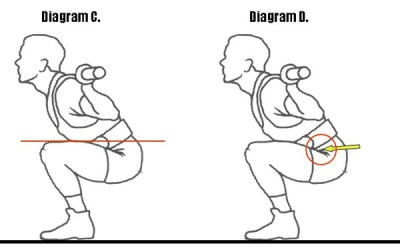
\includegraphics[width=0.8\linewidth]{squat-depth.jpg}

   \caption{Diagram of a squat considered to be ``depth."}
   \label{fig:onecol}
\end{figure}


%-------------------------------------------------------------------------